\documentclass[12 pt]{article}
\usepackage[utf8]{inputenc}
\usepackage{matlab-prettifier}
\usepackage[portuguese]{babel}
\usepackage{indentfirst}
\usepackage{graphicx}
\usepackage{float}
\usepackage{subcaption}
\usepackage[font=small,labelfont=bf]{caption}
\definecolor{mygreen}{RGB}{28,172,0} % color values Red, Green, Blue
\definecolor{myyellow}{rgb}{1.0, 1.0, 0.8}
\usepackage{mathtools}
\usepackage{multirow}
\usepackage{comment}
\usepackage{xcolor}
\usepackage{colortbl}
\usepackage[normalem]{ulem}               % to striketrhourhg text
\usepackage{amsmath}
\usepackage{amsfonts}
\usepackage{hyperref}
\usepackage{tcolorbox}
\tcbset{before upper={\setlength{\parindent}{2em}}}
\usepackage{longtable}
\usepackage{enumitem}


\newcommand\redout{\bgroup\markoverwith
{\textcolor{red}{\rule[0.5ex]{2pt}{0.8pt}}}\ULon}
\renewcommand{\lstlistingname}{Código}% Listing -> Algorithm
\renewcommand{\lstlistlistingname}{Lista de \lstlistingname s}% List of Listings -> List of Algorithms

\usepackage[top=3cm,left=2cm,bottom=2cm, right=2cm]{geometry}
\usepackage{tikz}
\usetikzlibrary{decorations.pathreplacing}
\usetikzlibrary{automata}
\usetikzlibrary{positioning}
\usetikzlibrary{arrows.meta, positioning}

\usepackage{adjustbox}

\usepackage{mdframed}
\newmdenv[
    backgroundcolor=gray!15,       % fundo cinza claro
    linecolor=gray!60,             % borda cinza mais escura
    linewidth=1pt,
    roundcorner=5pt,
    skipabove=10pt,
    skipbelow=10pt,
    innertopmargin=1em,
    innerbottommargin=1em,
    innerleftmargin=1em,
    innerrightmargin=1em,
    splittopskip=\topskip,
    firstextra=\setlength{\parindent}{2em}, 
]{respostabox@inner}

\newenvironment{resposta}
    {\begin{respostabox@inner}
    \setlength{\parindent}{2em}~
    }
  {\end{respostabox@inner}}

% Configuração para destacar a sintaxe do Python
\lstset{ 
    language=Python,                     % A linguagem do código
    backgroundcolor=\color{myyellow}, % A cor do fundo 
    basicstyle=\ttfamily\footnotesize,   % O estilo do texto básico
    keywordstyle=\color{blue},           % Cor das palavras-chave
    stringstyle=\color{red},             % Cor das strings
    commentstyle=\color{mygreen},          % Cor dos comentários
    numbers=left,                        % Números das linhas à esquerda
    numberstyle=\tiny\color{gray},       % Estilo dos números das linhas
    stepnumber=1,                        % Número de linhas entre os números das linhas
    frame=single,                        % Moldura ao redor do código
    breaklines=true,                     % Quebra automática das linhas longas
    captionpos=t,                        % Posição da legenda
    showstringspaces=false               % Não mostra espaços em branco nas strings
    extendedchars=true,
    literate={º}{{${ }^{\underline{o}}$}}1 {á}{{\'a}}1 {à}{{\`a}}1 {ã}{{\~a}}1 {é}{{\'e}}1 {É}{{\'E}}1 {ê}{{\^e}}1 {ë}{{\"e}}1 {í}{{\'i}}1 {ç}{{\c{c}}}1 {Ç}{{\c{C}}}1 {õ}{{\~o}}1 {ó}{{\'o}}1 {ô}{{\^o}}1 {ú}{{\'u}}1 {Ú}{{\'U}}1 {â}{{\^a}}1 {~}{{$\sim$}}1
}





\begin{document}


\noindent
\textbf{UFRJ / COPPE / PESC} \hfill \textbf{\today} \\



\begin{center}
CPS767 – \textit{Algoritmos de Monte Carlo e Cadeias de Markov}\\
\textbf{Prof.: Daniel Ratton Figueiredo} \\[1em]
\textbf{Aluno: Luiz Henrique Souza Caldas}\\ \texttt{lhscaldas@cos.ufrj.br} \\[1em]

\end{center}

\textbf{Proposta de Projeto:} Planejamento Dinâmico de Rotas para VANTs em Patrulha Naval

\vspace{1em}
\hrule
\vspace{2em}


\section{Motivação}
O Brasil possui uma extensa costa de 8{,}7 mil quilômetros, com 68 portos e uma faixa litorânea que concentra mais da metade da população e do PIB do país. Além disso, o país possui aproximadamente 4{,}5 milhões de quilômetros quadrados de águas jurisdicionais, onde se encontram recursos estratégicos como 95\% do petróleo e 83\% do gás natural nacionais, e por onde transitam cerca de 95\% do comércio exterior \cite{andrade_2021}.
Nesse contexto, a crescente adoção de Veículos Aéreos Não Tripulados (VANTs) em operações de vigilância marítima exige métodos mais robustos de planejamento de rotas, especialmente em cenários com alvos parcialmente conhecidos e detecção sensorial sujeita a limitações práticas. Trabalhos anteriores mostram que a vigilância baseada em varredura aérea pode ser modelada como uma variação do Problema do Caixeiro Viajante (TSP), incorporando restrições operacionais como autonomia limitada, sensores com alcances distintos e alvos móveis ou parcialmente observáveis \cite{marlow_2007}.
Técnicas de otimização como o \textit{Simulated Annealing} têm se mostrado eficazes em problemas de roteamento com grande espaço de busca e múltiplos mínimos locais, sendo uma escolha promissora para o replanejamento progressivo de trajetos em ambientes com inserção dinâmica de alvos \cite{kosmas_2012}.
Mais recentemente, abordagens com replanejamento dinâmico em tempo real vêm sendo propostas para garantir a cobertura de alvos não detectados ou mal inspecionados, especialmente em aplicações com VANTs e sensores embarcados \cite{penicka_2017}. Motivado por esses avanços, este trabalho propõe uma formulação adaptada do TSP para missões de patrulha marítima com inserção condicional de novos alvos, levando em conta restrições de distância lateral, autonomia do VANT e alcance heterogêneo de sensores.

\begin{figure}[H]
    \centering
    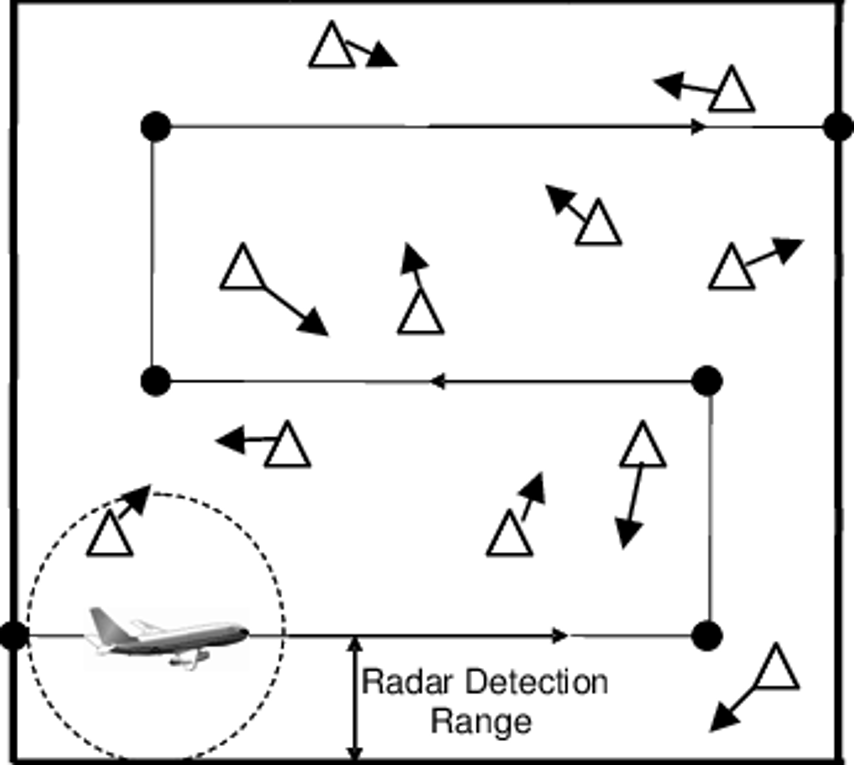
\includegraphics[width=0.6\textwidth]{fig/vant.png}
    \caption{Patrulha naval realizada por aeronave.}

    \small
    \textbf{Fonte:} Marlow et al 2007 \cite{marlow_2007}.
 \end{figure}

\section{Objetivo}
O objetivo deste trabalho é desenvolver uma metodologia para o planejamento dinâmico de rotas de VANTs em missões de vigilância marítima, considerando a detecção progressiva de alvos ao longo do percurso. A proposta visa adaptar o Problema do Caixeiro Viajante (TSP) a um contexto em que novos pontos de interesse são identificados durante a missão, e a decisão de incluí-los no trajeto deve considerar restrições operacionais e de sensoriamento. A solução deve permitir o replanejamento eficiente da rota, de forma a maximizar a inspeção de alvos relevantes, respeitando os limites de autonomia da aeronave.

\section{Metodologia}
A metodologia proposta consiste na varredura da área marítima por um VANT que percorre linhas paralelas, com waypoints pré-definidos. O VANT está equipado com sensores de detecção, incluindo um radar com alcance \( R_{\text{radar}} \) e uma câmera de identificação visual com alcance \( R_{\text{câmera}} \), ambos tratados como parâmetros configuráveis. Durante o voo, sempre que o radar detecta um novo navio, sua posição é considerada um \textit{vértice candidato} no grafo de inspeção.

Contudo, para evitar grandes desvios do padrão de varredura, esse ponto só é efetivamente adicionado se a distância perpendicular entre o navio e a linha paralela atualmente seguida pelo VANT for inferior a uma distância configurável \(d\). Essa restrição evita que o VANT se afaste excessivamente do percurso principal para inspecionar alvos muito distantes lateralmente.

À medida que novos vértices são inseridos, o problema de roteamento é resolvido incrementalmente por meio do algoritmo de \textit{Simulated Annealing}, uma metaheurística eficaz para encontrar boas soluções aproximadas em instâncias complexas do Problema do Caixeiro Viajante. O objetivo é minimizar a distância total percorrida, respeitando a autonomia máxima do VANT e maximizando o número de alvos inspecionados de acordo com os critérios definidos.

Como simplificação, assume-se que os navios estão estáticos durante a missão, dada a superioridade da velocidade do VANT em relação às embarcações. Essa modelagem permite representar o problema como um TSP com inserção condicional de vértices durante a missão.

\section{Resultados Esperados}
Espera-se, com essa abordagem, obter um modelo que equilibre eficiência de cobertura com esforço computacional, além de fornecer uma solução aplicável em cenários operacionais reais. A contribuição principal está na integração de critérios práticos de operação com modelos clássicos de otimização, promovendo maior aderência do TSP a situações reais de patrulhamento com VANTs.


\bibliographystyle{abntex2-num}
\bibliography{bibliografia}

\end{document}